\section{Datasets and experimental setup}
\begin{longtable}{lrrrrrr}
\caption{Frozen task datasets and literal positive counts.}\label{tab:datasets}\\
\toprule
Dataset & Rows & TRAIN & TEST & TRAIN+ & TEST+ & Candidates \\
\midrule
\endfirsthead
\toprule
Dataset & Rows & TRAIN & TEST & TRAIN+ & TEST+ & Candidates \\
\midrule
\endhead
Abalone19 & 4174 & 3340 & 834 & 26 & 6 & 200 \\
Ecoli4 & 336 & 269 & 67 & 16 & 4 & 201 \\
page-blocks0 & 5472 & 4377 & 1095 & 447 & 112 & 200 \\
\bottomrule
\end{longtable}

Only existing datasets/splits are used. Abalone19 has seven numerical and one nominal feature; Ecoli4 seven numerical; page-blocks0 ten numerical. Positive/negative are literal tokens, not inferred physical meanings. Few TEST positives make metrics sensitive. Historical exact-value TRAIN/TEST overlap is disclosed: disjoint row identities do not imply independent values.

Phase 3 records five configurations with 1,803 evidence rows each. Phase 4 records six policies. Phase 5 records 51 datasets: four-strategy/three-budget comparisons, B2-intersection controls and cutoff sensitivities. Budgets derive in advance from fractions $.25,.50,.75$ of distinct eligible feature count: 28/56/84, 35/70/105 and 24/49/74. Phase 6 compares original/augmented pools at middle budgets, producing 24 constructions. No new providers, datasets or families are introduced.

\subsection{Baselines and task-utility protocol}
\begin{longtable}{lrrrr}
\caption{Recorded control acceptance and separately named complete structure-compatible utility subsets. Acceptance is not verified validity.}\label{tab:controls}\\
\toprule
Dataset / control & Accepted & Candidates & Utility subset & Pass difference \\
\midrule
\endfirsthead
\toprule
Dataset / control & Accepted & Candidates & Utility subset & Pass difference \\
\midrule
\endhead
Abalone19 / B1 & 200 & 200 & 195 & 30 \\
Abalone19 / B2 & 138 & 200 & 138 & 78 \\
Abalone19 / B3 & 200 & 200 & 195 & 30 \\
Ecoli4 / B1 & 201 & 201 & 195 & 39 \\
Ecoli4 / B2 & 174 & 201 & 174 & 54 \\
Ecoli4 / B3 & 200 & 201 & 195 & 38 \\
page-blocks0 / B1 & 200 & 200 & 136 & 81 \\
page-blocks0 / B2 & 175 & 200 & 116 & 96 \\
page-blocks0 / B3 & 200 & 200 & 136 & 81 \\
\bottomrule
\end{longtable}

New utility controls intersect recorded B1/B2/B3 acceptance with complete structure-compatible payloads. Filtering is named, not a redefinition of raw controls. Historical integration forms a DataFrame directly from candidate data; missing class can become NaN then the string \texttt{nan} in its scorer. Historical unfiltered results remain preserved, not silently endorsed as complete binary-record comparisons.

TRTR trains real TRAIN; TSTR synthetic data only; HYBRID\_MINORITY real TRAIN plus synthetic positive-literal records. One-class synthetic data makes binary TSTR unavailable. No minority augmentation makes hybrid unavailable, not relabeled TRTR. No invalid records or invented labels create balance.

Reuse frozen median-imputation, scaling and nominal encoding fitted on each actual training population. Models are logistic regression (liblinear, maximum 300 iterations) and 50-tree random forest, seed 42. The full matrix was committed before TEST scoring: two TRTR rows per dataset plus eleven sources, two models and two regimes, totaling 138. Models, metrics, rules and budgets were fixed before scores.

Historical generation/evidence/selection use full TRAIN. An inner holdout would not be independent without rebuilding upstream steps; none is claimed. Comparisons use previously evaluated outer TEST descriptively. TEST never fits evidence, transformations, repair, selection, preprocessing or classifiers. No TEST-driven tuning follows. One split/seed is studied; replay is not repetition.

\subsection{Metrics}
For positive-literal confusion counts,
\begin{align}
F_1&=\frac{2TP}{2TP+FP+FN},&
BA&=\frac12\left(\frac{TP}{TP+FN}+\frac{TN}{TN+FP}\right),\\
MCC&=\frac{TP\,TN-FP\,FN}{\sqrt{(TP+FP)(TP+FN)(TN+FP)(TN+FN)}}.
\end{align}
Average precision is $AP=\sum_k(R_k-R_{k-1})P_k$; \texttt{pr\_auc} is an AP alias, not trapezoidal PR area. AUROC measures positive/negative ordering with half credit for ties. Undefined metrics retain reason/null behavior. These are task metrics, not human validity or agreement.

\section{Results}
\subsection{Structural evidence and dependence}
\begin{longtable}{lrrrrr}
\caption{Baseline local/global dependence and concern disagreement at descriptive cutoff .90.}\label{tab:evidence}\\
\toprule
Dataset & Paired & Spearman & Union & Intersection & Disagree \\
\midrule
\endfirsthead
\toprule
Dataset & Paired & Spearman & Union & Intersection & Disagree \\
\midrule
\endhead
Abalone19 & 200 & 0.9076 & 27 & 13 & 14 \\
Ecoli4 & 200 & 0.4876 & 35 & 5 & 30 \\
page-blocks0 & 200 & 0.6205 & 21 & 19 & 2 \\
\bottomrule
\end{longtable}

Local/global evidence is highly dependent for Abalone19 and moderately correlated for the others, with distinct tail overlaps. Structural/B2 disagreements total 157; without human truth they are predicate disagreements, not model errors. Local/global evidence is available for 600 payloads; one Ecoli4 record lacks seven features.

\begin{longtable}{lrrrr}
\caption{Frozen exploratory policies. R: structural reject; V: review; P: provisional pass; A: abstain.}\label{tab:shadow}\\
\toprule
Dataset / policy & R & V & P & A \\
\midrule
\endfirsthead
\toprule
Dataset / policy & R & V & P & A \\
\midrule
\endhead
Abalone19 / combined-review & 5 & 25 & 170 & 0 \\
Abalone19 / combined-review-q80 & 5 & 47 & 148 & 0 \\
Abalone19 / combined-review-q95 & 5 & 11 & 184 & 0 \\
Abalone19 / global-review & 5 & 18 & 177 & 0 \\
Abalone19 / local-review & 5 & 18 & 177 & 0 \\
Abalone19 / structure-only & 5 & 0 & 195 & 0 \\
Ecoli4 / combined-review & 6 & 33 & 162 & 0 \\
Ecoli4 / combined-review-q80 & 6 & 64 & 131 & 0 \\
Ecoli4 / combined-review-q95 & 6 & 17 & 178 & 0 \\
Ecoli4 / global-review & 6 & 18 & 177 & 0 \\
Ecoli4 / local-review & 6 & 20 & 175 & 0 \\
Ecoli4 / structure-only & 6 & 0 & 195 & 0 \\
page-blocks0 / combined-review & 64 & 17 & 119 & 0 \\
page-blocks0 / combined-review-q80 & 64 & 39 & 97 & 0 \\
page-blocks0 / combined-review-q95 & 64 & 10 & 126 & 0 \\
page-blocks0 / global-review & 64 & 16 & 120 & 0 \\
page-blocks0 / local-review & 64 & 16 & 120 & 0 \\
page-blocks0 / structure-only & 64 & 0 & 136 & 0 \\
\bottomrule
\end{longtable}

Combined $.90$ produces 451 provisional passes, 75 structural rejects and 75 review-required records. Sensitivities remain exploratory alternatives. No policy is declared scientifically optimal.

\subsection{Construction and bounded repair}
Source-order selection can omit minority records at matched budgets, making TSTR/augmentation unavailable. Weighting, quotas and diversity change distinct properties. The appendix gives primary budgets; all 51 original audits remain in their manifest.

\begin{longtable}{lrrrrr}
\caption{Approved integer-only repair outcomes; denominator is original structural rejects.}\label{tab:repair}\\
\toprule
Dataset & Rejects & Eligible & Applied & Failed & Ineligible \\
\midrule
\endfirsthead
\toprule
Dataset & Rejects & Eligible & Applied & Failed & Ineligible \\
\midrule
\endhead
Abalone19 & 5 & 0 & 0 & 0 & 5 \\
Ecoli4 & 6 & 0 & 0 & 0 & 6 \\
page-blocks0 & 64 & 54 & 54 & 0 & 10 \\
\bottomrule
\end{longtable}

Fifteen records lack class, one lacks features, and 64 have fractional integer fields; categories overlap. Twenty-six have multiple field violations. No invalid-primitive or unsupported-nominal case occurs here. Of fractional-field records, five also lack class and five require over three edits; ten are ineligible. Eleven further ineligible records belong to the other datasets.

Figure~\ref{fig:repair} summarizes the outcomes. The 54 repairs edit 73 fields: 39 records need one edit, eleven two, four three. Changes range .1--.5, mean .3119, median .2. All become structurally compatible; 49 are provisional and five require review. Originals retain prior decisions. Restored M2 reproduces original evidence exactly, with zero maximum raw-score difference. No fitting/reranking occurs.

\begin{figure}[ht]\centering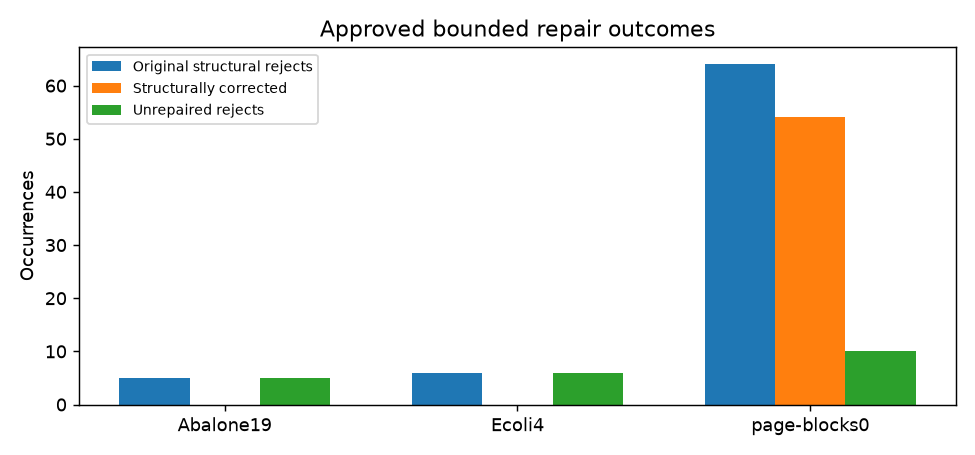
\includegraphics[width=.85\linewidth]{figures/repair-outcomes.png}\caption{Repair outcomes by original occurrence; structural correction is not human validity.}\label{fig:repair}\end{figure}
The largest observed absolute percentile shift is .0275 locally: page-blocks0 source occurrence 131 rounds height 4.5 to 4 and Lenght 32.5 to 32. Global percentile changes .0075; its action becomes provisional pass. This pool supplies no extreme evidence discontinuity. The report lists largest observed shifts without manufacturing a dramatic example.

\small\begin{longtable}{lrrrrr}
\caption{Matched middle-budget construction. C: distinct-feature TRAIN coverage; D: exact duplicate rate; N: near-duplicate rate. O: original pool; R: repair-augmented pool.}\label{tab:coverage}\\
\toprule
Dataset / strategy / pool & n & Derived & C & D & N \\
\midrule
\endfirsthead
\toprule
Dataset / strategy / pool & n & Derived & C & D & N \\
\midrule
\endhead
page-blocks0 / source-order / O & 49 & 0 & 0.9139 & 0.2653 & 0.5918 \\
page-blocks0 / source-order / R & 49 & 11 & 0.9099 & 0.1837 & 0.5918 \\
page-blocks0 / farthest-first / O & 49 & 0 & 0.9324 & 0.0000 & 0.0000 \\
page-blocks0 / farthest-first / R & 49 & 11 & 0.9359 & 0.0000 & 0.0000 \\
page-blocks0 / coverage-greedy / O & 49 & 0 & 0.9324 & 0.1633 & 0.4490 \\
page-blocks0 / coverage-greedy / R & 49 & 9 & 0.9370 & 0.0816 & 0.4082 \\
page-blocks0 / quality-coverage / O & 49 & 0 & 0.9324 & 0.0000 & 0.3265 \\
page-blocks0 / quality-coverage / R & 49 & 16 & 0.9370 & 0.0000 & 0.1020 \\
Ecoli4 / source-order / O & 70 & 0 & 0.4164 & 0.2000 & 0.3857 \\
Ecoli4 / source-order / R & 70 & 0 & 0.4164 & 0.2000 & 0.3857 \\
Ecoli4 / farthest-first / O & 70 & 0 & 0.4684 & 0.0000 & 0.0000 \\
Ecoli4 / farthest-first / R & 70 & 0 & 0.4684 & 0.0000 & 0.0000 \\
Ecoli4 / coverage-greedy / O & 70 & 0 & 0.5056 & 0.1143 & 0.2429 \\
Ecoli4 / coverage-greedy / R & 70 & 0 & 0.5056 & 0.1143 & 0.2429 \\
Ecoli4 / quality-coverage / O & 70 & 0 & 0.5056 & 0.0000 & 0.0000 \\
Ecoli4 / quality-coverage / R & 70 & 0 & 0.5056 & 0.0000 & 0.0000 \\
Abalone19 / source-order / O & 56 & 0 & 0.6225 & 0.3571 & 0.6250 \\
Abalone19 / source-order / R & 56 & 0 & 0.6225 & 0.3571 & 0.6250 \\
Abalone19 / farthest-first / O & 56 & 0 & 0.9401 & 0.0000 & 0.0000 \\
Abalone19 / farthest-first / R & 56 & 0 & 0.9401 & 0.0000 & 0.0000 \\
Abalone19 / coverage-greedy / O & 56 & 0 & 0.9479 & 0.1071 & 0.2679 \\
Abalone19 / coverage-greedy / R & 56 & 0 & 0.9479 & 0.1071 & 0.2679 \\
Abalone19 / quality-coverage / O & 56 & 0 & 0.9479 & 0.0000 & 0.0000 \\
Abalone19 / quality-coverage / R & 56 & 0 & 0.9479 & 0.0000 & 0.0000 \\
\bottomrule
\end{longtable}
\normalsize
Figure~\ref{fig:coverage} compares geometric coverage. The pool grows 451 to 500 through page-blocks0 (119 to 168). Original conditions exactly reproduce Phase 5. At page budget 49, quality-coverage selects 16 derived records: distinct-feature TRAIN coverage rises .9324 to .9370, near duplication falls .3265 to .1020, exact duplication remains zero. Source-order coverage slightly declines. Pool expansion does not guarantee a better fixed-budget set. The other datasets stay unchanged.

\begin{figure}[ht]\centering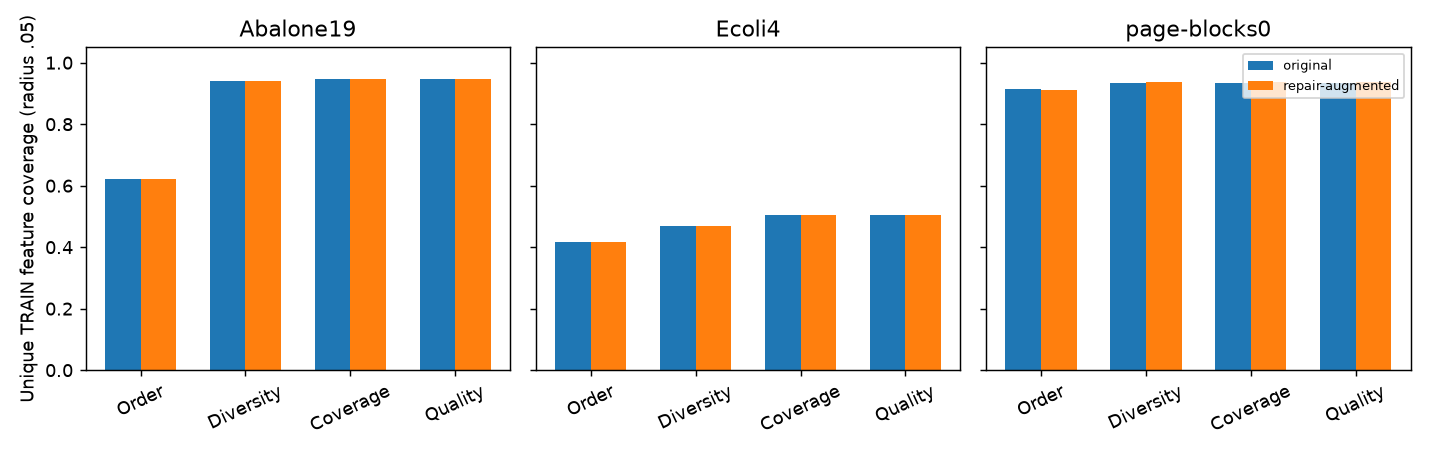
\includegraphics[width=\linewidth]{figures/coverage-comparison.png}\caption{Matched budgets; coverage describes TRAIN geometry, not accuracy.}\label{fig:coverage}\end{figure}

\subsection{Task utility and unavailable comparisons}
\small\begin{longtable}{lrrrr}
\caption{Fixed TEST task utility. L/F: logistic/random forest. QO/QR: quality-coverage original/repair pool. H: hybrid minority augmentation.}\label{tab:utility}\\
\toprule
Dataset / source / regime / model & F1 & AP & BA & MCC \\
\midrule
\endfirsthead
\toprule
Dataset / source / regime / model & F1 & AP & BA & MCC \\
\midrule
\endhead
Abalone19 / Real / TRTR / L & 0.0000 & 0.0256 & 0.5000 & 0.0000 \\
Abalone19 / Real / TRTR / F & 0.0000 & 0.0231 & 0.5000 & 0.0000 \\
Abalone19 / QO / TSTR / L & 0.0312 & 0.0191 & 0.7748 & 0.0933 \\
Abalone19 / QO / H / L & 0.0000 & 0.0170 & 0.5000 & 0.0000 \\
Abalone19 / QO / TSTR / F & 0.0303 & 0.0211 & 0.7240 & 0.0777 \\
Abalone19 / QO / H / F & 0.0000 & 0.0365 & 0.4994 & -0.0029 \\
Abalone19 / QR / TSTR / L & 0.0312 & 0.0191 & 0.7748 & 0.0933 \\
Abalone19 / QR / H / L & 0.0000 & 0.0170 & 0.5000 & 0.0000 \\
Abalone19 / QR / TSTR / F & 0.0303 & 0.0211 & 0.7240 & 0.0777 \\
Abalone19 / QR / H / F & 0.0000 & 0.0365 & 0.4994 & -0.0029 \\
Ecoli4 / Real / TRTR / L & 1.0000 & 1.0000 & 1.0000 & 1.0000 \\
Ecoli4 / Real / TRTR / F & 0.6667 & 1.0000 & 0.7500 & 0.6961 \\
Ecoli4 / QO / TSTR / L & 0.2051 & 0.1355 & 0.7540 & 0.2409 \\
Ecoli4 / QO / H / L & 1.0000 & 1.0000 & 1.0000 & 1.0000 \\
Ecoli4 / QO / TSTR / F & 0.2963 & 0.6326 & 0.8492 & 0.3485 \\
Ecoli4 / QO / H / F & 1.0000 & 1.0000 & 1.0000 & 1.0000 \\
Ecoli4 / QR / TSTR / L & 0.2051 & 0.1355 & 0.7540 & 0.2409 \\
Ecoli4 / QR / H / L & 1.0000 & 1.0000 & 1.0000 & 1.0000 \\
Ecoli4 / QR / TSTR / F & 0.2963 & 0.6326 & 0.8492 & 0.3485 \\
Ecoli4 / QR / H / F & 1.0000 & 1.0000 & 1.0000 & 1.0000 \\
page-blocks0 / Real / TRTR / L & 0.7150 & 0.7456 & 0.8019 & 0.6991 \\
page-blocks0 / Real / TRTR / F & 0.8692 & 0.9213 & 0.9106 & 0.8562 \\
page-blocks0 / QO / TSTR / L & 0.4464 & 0.5552 & 0.7590 & 0.3892 \\
page-blocks0 / QO / H / L & 0.7150 & 0.7444 & 0.8019 & 0.6991 \\
page-blocks0 / QO / TSTR / F & 0.3421 & 0.4468 & 0.7269 & 0.2880 \\
page-blocks0 / QO / H / F & 0.8626 & 0.9094 & 0.9022 & 0.8499 \\
page-blocks0 / QR / TSTR / L & 0.3421 & 0.5716 & 0.7129 & 0.2780 \\
page-blocks0 / QR / H / L & 0.7150 & 0.7423 & 0.8019 & 0.6991 \\
page-blocks0 / QR / TSTR / F & 0.3158 & 0.4742 & 0.7041 & 0.2544 \\
page-blocks0 / QR / H / F & 0.8732 & 0.9093 & 0.9111 & 0.8610 \\
\bottomrule
\end{longtable}
\normalsize
Of 138 rows, 114 return results and 24 are unavailable. The six source-order populations, each with two models/two regimes, contain no positive-literal synthetic records. No favorable substitute replaces an unavailable result. Full controls and other strategies remain in CSV/JSON.

Figure~\ref{fig:utility} shows the fixed logistic comparisons. Abalone19 TRTR F1 is zero for both models despite nonzero ranking metrics. Ecoli4 logistic TRTR reaches 1.0 on only four TEST positives, not proof of universal performance. Page quality-coverage logistic TSTR F1 falls .4464 to .3421 after repair-pool expansion while AP rises .5552 to .5716. Hybrid F1 remains .7150 and AP slightly falls. These mixed outcomes do not establish uniform improvement. No significance/interval is inferred from one split.

\begin{figure}[ht]\centering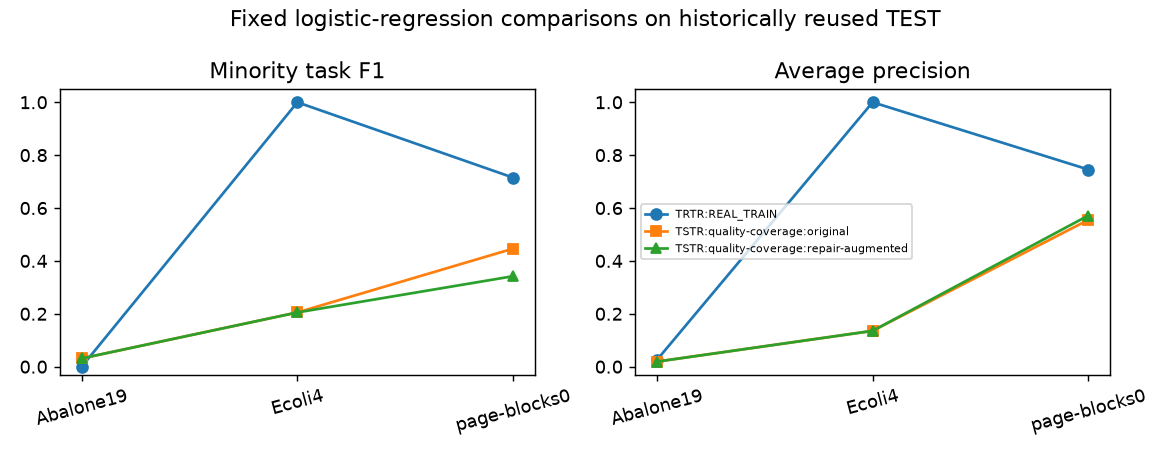
\includegraphics[width=\linewidth]{figures/task-utility.png}\caption{Fixed logistic comparisons on reused historical TEST. Connected points identify datasets, not an ordered trend.}\label{fig:utility}\end{figure}

\subsection{Reproducibility and runtime}
Repair records, constructions and task payloads replay exactly in new locations. Runtime envelopes need not share fingerprints; substantive content does. M2 replay covers 601 occurrences/three families. The registry contains 258 entries across controls, configurations, policies, original constructions, repair, new constructions and utility. Original 51-dataset audit evidence is retained rather than rerun.

Repair scoring takes about 2.590 seconds on this workstation, excluding context loading/construction. Utility runtime and dependencies are recorded; no hardware-general speed claim is made. Replay supplies no confidence interval. Final tests, static checks and historical hashes are recorded separately in closeout evidence.
